\section{Diseño y resolución}

En este apartado vamos a pasar a explicar los detalles del desarrollo del proyecto. Como se ha dicho, el proyecto consiste en realizar un sistema capaz de seguir los movimientos del balón y las jugadoras de un partido de volleyball mediante imágenes proporcionadas por una cámara en vista cenital.

El seguimiento se puede realizar por \textit{tracking}, sustracción de fondo, o bien un sistema que aúne ambas cosas para una mayor robustez.

Una vez resuelta la parte del seguimiento, el siguiente objetivo sería registrar las posiciones detectadas a un fichero de salida en formato CSV, mediante el cual se puedan hacer análisis de distintas métricas del juego.

El desarrollo se va a centrar, como he ido aclarando, en una aplicación en Python utilizando OpenCV y PyQt para la parte de interfaz gráfica. De cara a la construcción del sistema, la estrategia a seguir es desarrollar separadamente sus partes y posteriormente implementarlas para que funcionen de manera conjunta.

A continuación detallaré estas partes y cómo se ha resuelto su implementación. Las partes principales del sistema son: sustracción de fondo, seguimiento (\textit{tracking}), interfaz gráfica y métodos de consistencia temporal

\subsection{Sustracción de fondo}
Para empezar a detectar formas en la imagen, primero nuestro sistema tiene que ser capaz de hacer una estimación del fondo. La técnica mediante la cual se hace esto se denomina sustracción de fondo. Esta es, por tanto, una parte primordial de nuestro sistema que debe funcionar de una manera suficientemente robusta. Este debe ser capaz, además, de distinguir a las jugadoras del balón, y de etiquetar cada una de las formas de una manera consistente entre los frames del vídeo.

\begin{figure}
    \centering
    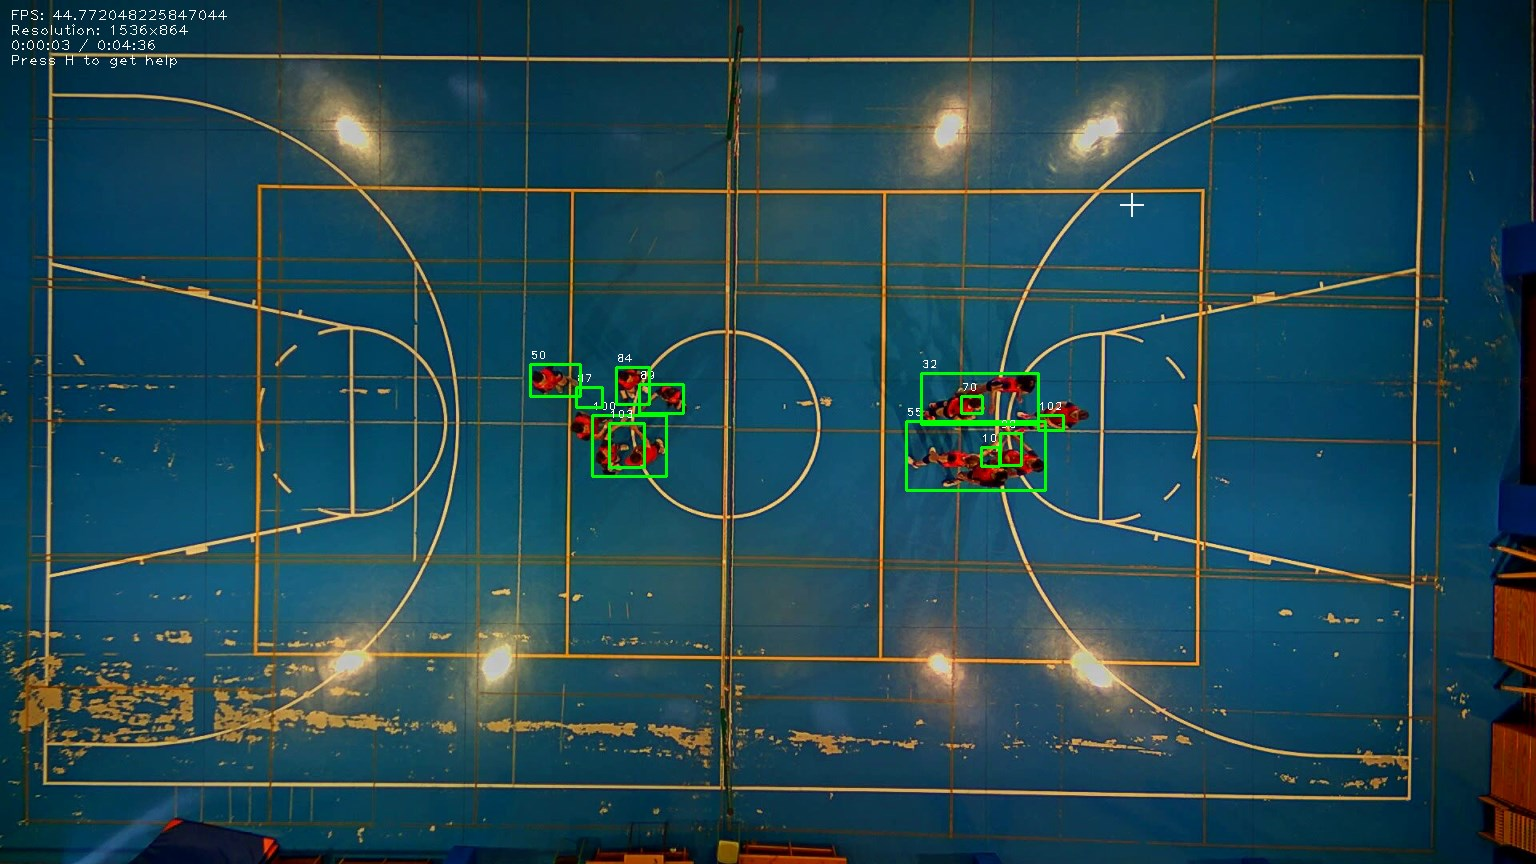
\includegraphics[width=0.5\textwidth]{images/nonms}
    \caption{Imagen de salida sin la operación de supresión de máximos}
    \label{fig:nonms}
\end{figure}

\begin{figure}
    \centering
    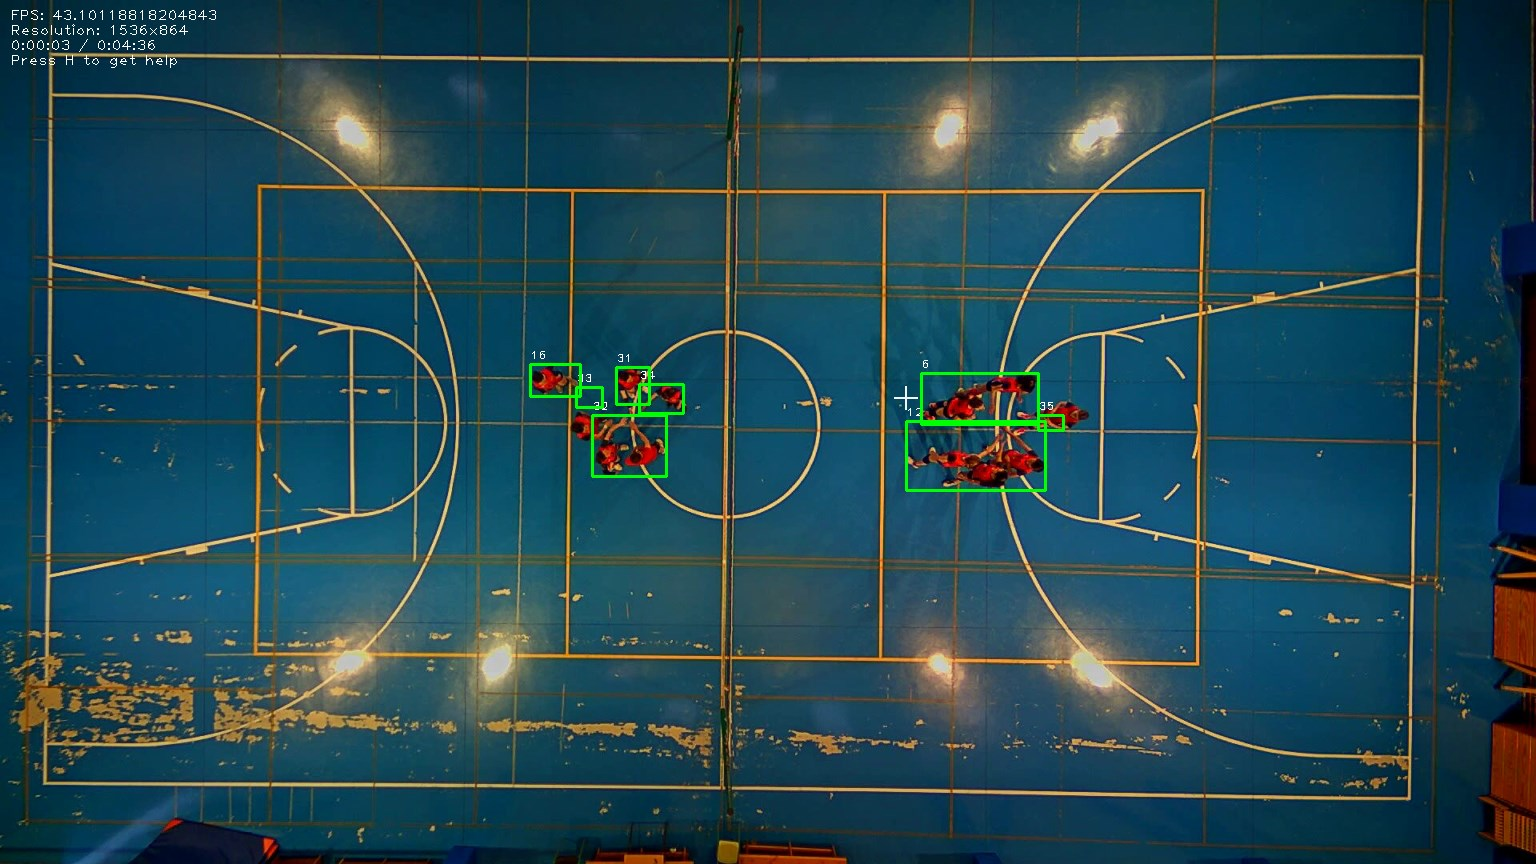
\includegraphics[width=0.5\textwidth]{images/nms}
    \caption{Imagen de salida tras la operación de supresión de máximos}
    \label{fig:nms}
\end{figure}

Para ello, tras detectar las formas que forman parte del primer plano de la imagen se realizan una serie de operaciones. La primera de ellas es la \textbf{supresión de no máximos}. En ciertos momentos del vídeo, puede que no se detecte una forma de manera completa, sino que se detecta el contorno y ciertas partes separadas. Cuando esto ocurre, la imagen de salida tiene la forma que vemos en la figura \ref{fig:nonms} donde pueden verse varios cuadrados redundantes que podrían englobarse en uno más grande. Tras aplicar la supresión de no máximos, la imagen queda como en la figura \ref{fig:nms}, donde puede verse que los cuadrados contenidos dentro de otros han sido suprimidos.

La segunda operación es el \textbf{test de circularidad}, el cual nos sirve para saber cuál de las formas detectadas en la imagen es el balón. Para ello, calculamos el coeficiente de circularidad $C =  \frac{4*\pi*\acute{a}rea}{per\acute{\imath}metro^2}$. Cuanto mayor sea $C$, mayor probabilidad de que la forma sea la de un círculo, es decir, la del balón. En un frame cualquiera, la forma cuyo coeficiente $C$ tenga un valor mayor de 0.6 y sea el mayor de todos los contornos detectados, se marcará en rojo en la imagen de salida, mientras que el resto se marcarán en verde.

La última de las operaciones que se realizan es el etiquetado de los contornos detectados. Esto es importante ya que de un frame a otro, no tenemos una manera rápida de saber qué contorno del frame actual corresponde con qué contorno del anterior. Para solucionar esta problemática, en el primer frame se da una etiqueta a todos los contornos que se detecta. A partir de aquí, en los siguientes frames se irá etiquetando en base a un emparejamiento mutuo entre los contornos, calculando una matriz de distancias de todos los contornos entre sí. Una vez calculada esta matriz, si para un contorno $c$, su más cercano es otro contorno $k$ y si para $k$ el mas cercano es $c$, esto quiere decir que son el mismo contorno. En caso de quedar contornos sin pareja después de esto, simplemente se les da una etiqueta nueva

Una vez establecidas estas operaciones secundarias, tenemos que solucionar el problema principal, la sustracción de fondo. Teniendo en cuenta que las imágenes proceden de una cámara fija y cenital, y que por tanto el fondo siempre va a ser exactamente el mismo, una primera aproximación ingenua a este problema podría ser tan simple como realizar una diferencia entre los frames del video.

Por desgracia, las condiciones de iluminación no siempre van a ser totalmente iguales, lo cual va a dificultar en gran medida la detección de objetos usando este método. Además, no siempre vamos a tener disponible una imagen limpia del campo en un vídeo para usar como modelo de fondo. Por ello es complicado realizar un modelo del campo para las diferentes condiciones de iluminación a lo largo de un día mediante resta de frames.

Ademas de la sensibilidad a cambios en la iluminación, este método adolece de otra desventaja: no es capaz de detectar sombras. Las imágenes que usamos son las de un campo de volleyball dentro de un pabellón, y los focos de dentro de este hacen que sea bastante común tener sombras alargadas y notables en las jugadoras.

Una vez hemos podido ver que esta manera de proceder no es todo lo viable que cabría desear, tendremos que empezar a plantearnos otras opciones a nuestra disposición. OpenCV proporciona distintos algoritmos de sustracción de fondo, los cuales podemos aprovechar y comparar para ver cuál es más apropiado en nuestro propósito.

\begin{figure}
    \centering
    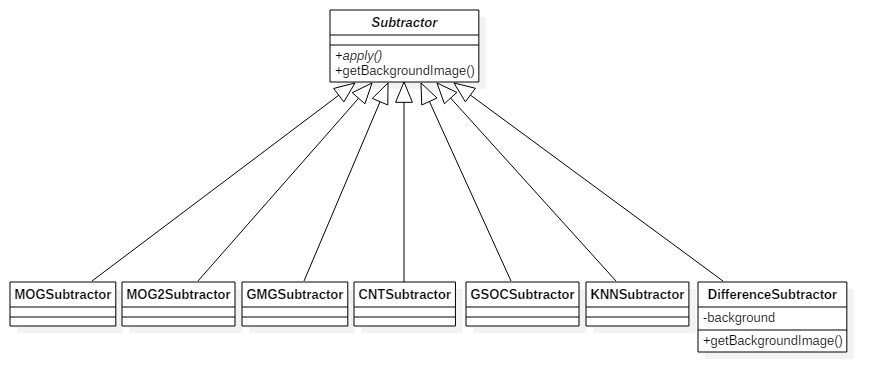
\includegraphics[width=0.9\textwidth]{images/subtractors}
    \caption{Estructura de clases de los sustractores de fondo}
    \label{fig:subtractors}
\end{figure}

Para facilitar el uso de estos algoritmos, se ha hecho uso de la programación orientada a objetos que nos ofrece Python. Se ha creado una clase abstracta llamada Subtractor de la cual heredan todas las clases que hagan uso de los algoritmos de OpenCV así como el de diferencia de frames. Dicha clase proporciona una interfaz común a todas las clases, que hará mas sencillo el uso de ellas. La estructura resultante puede verse en la figura \ref{fig:subtractors}.

El funcionamiento interno de las clases resultantes, como se ha dicho, corresponde a las propias implementaciones de OpenCV. Pasaré a explicar los fundamentos teóricos de cada uno de estos algoritmos.

\subsubsection*{MOG}
MOG, mezcla de gaussianas (\textit{Mixture of Gaussians}), fue descrito en  \cite{KaewTraKulPong2002} partiendo de otro algoritmo ya existente de Grimson \textit{et al} \cite{698583,784637,868677}. Ambas versiones crean un modelo del fondo en base a una mezcla de k gaussianas con $3\leq k \leq 5$, cada una de las cuales representa un color. La probabilidad de que un pixel tenga el valor $x_N$ en tiempo N es de
\[
    p(x_N) = \sum_{j=1}^{k} w_j \eta (x_N;\theta_j )
\]
donde $w_k$ es el peso de la componente guasiana k-ésima. $\theta(x;\theta_k)$ es la ecuación que define la distribución de la componente, representada por
\[
    \theta(x;\theta_k) = \theta(x;\mu_k, \Sigma_k) = \frac{1}{(2\pi)^{\frac{D}{2}}|\Sigma_k|^\frac{1}{2}}e^{-\frac{1}{2}(x-\mu_k)^T\Sigma_k^{-1}(x-\mu_k)}
\]
donde $\mu_k$ es la media y $\Sigma = \sigma_k^2I$ es la covarianza de la componente. Las distribuciones se ordenan en base a su fitness, definido por $\frac{w_k}{\sigma_k}$ y las B primeras son el modelo de fondo con $B = \arg\min (\sum_{j=1}^{k} w_j < T)$ donde T es el límite de probabilidad mínima a partir de cual un pixel se considera fondo. Un pixel se considera parte de los objetos de la escena si está 2.5 desviaciones por encima de una de las B distribuciones.

La diferencia entre la implementación original de Grimson y la de este algoritmo es las funciones de actualización de cada frame. En el caso del original las funciones de actualización son: 
\begin{align*}
    &\hat{w}_k^{N+1} = (1 - \alpha)\hat{w}_k^{N} + \alpha\hat{p}(\omega_k | x_{N+1}) \\
    &\hat{\mu}_k^{N+1} = (1 - \alpha)\hat{\mu}_k^{N} + \rho x_{N+1} \\
    &\hat{\Sigma}_k^{N+1} = (1 - \alpha)\hat{\Sigma}_k^{N} + \rho (x_{N+1} - \hat{\mu}_k^{N+1})(x_{N+1} - \hat{\mu}_k^{N+1})^T \\
    &\rho = \alpha \eta(x_{N+1};\hat{\mu}_k^N, \hat{\Sigma}_k^N) \\
    &\hat{p}(\omega_k | x_{N+1}) = \text{1 si $\omega_k$ es la primera componente gaussiana; 0 si no}
\end{align*}

%Version expected sufficient statistics

%Versión L- recent

Una novedad de MOG respecto a su predecesor es la capacidad para discernir las sombras de los objetos que las proyectan. Para ello se emplea una diferencia de la componente cromática y del brillo y si pasa de ciertos límites, se marca como sombra. Más concretamente, %ecuaciones de sombras

\begin{figure}
\begin{subfigure}{.5\textwidth}
  \centering
  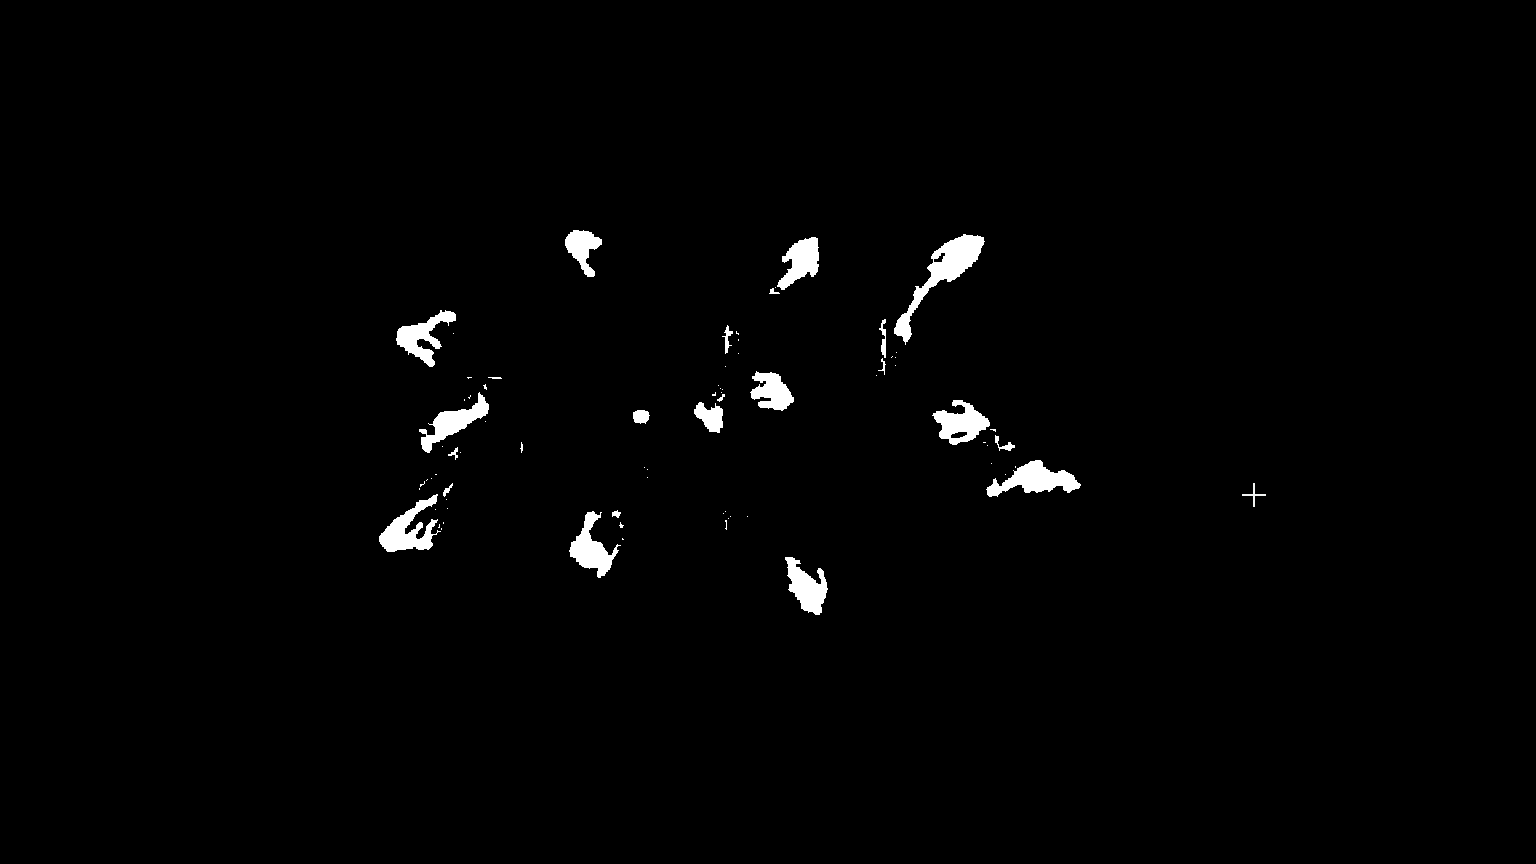
\includegraphics[width=.9\linewidth]{images/MOGsub}
  \caption { }
  \label{fig:MOG1a}
\end{subfigure}%
\begin{subfigure}{.5\textwidth}
  \centering
  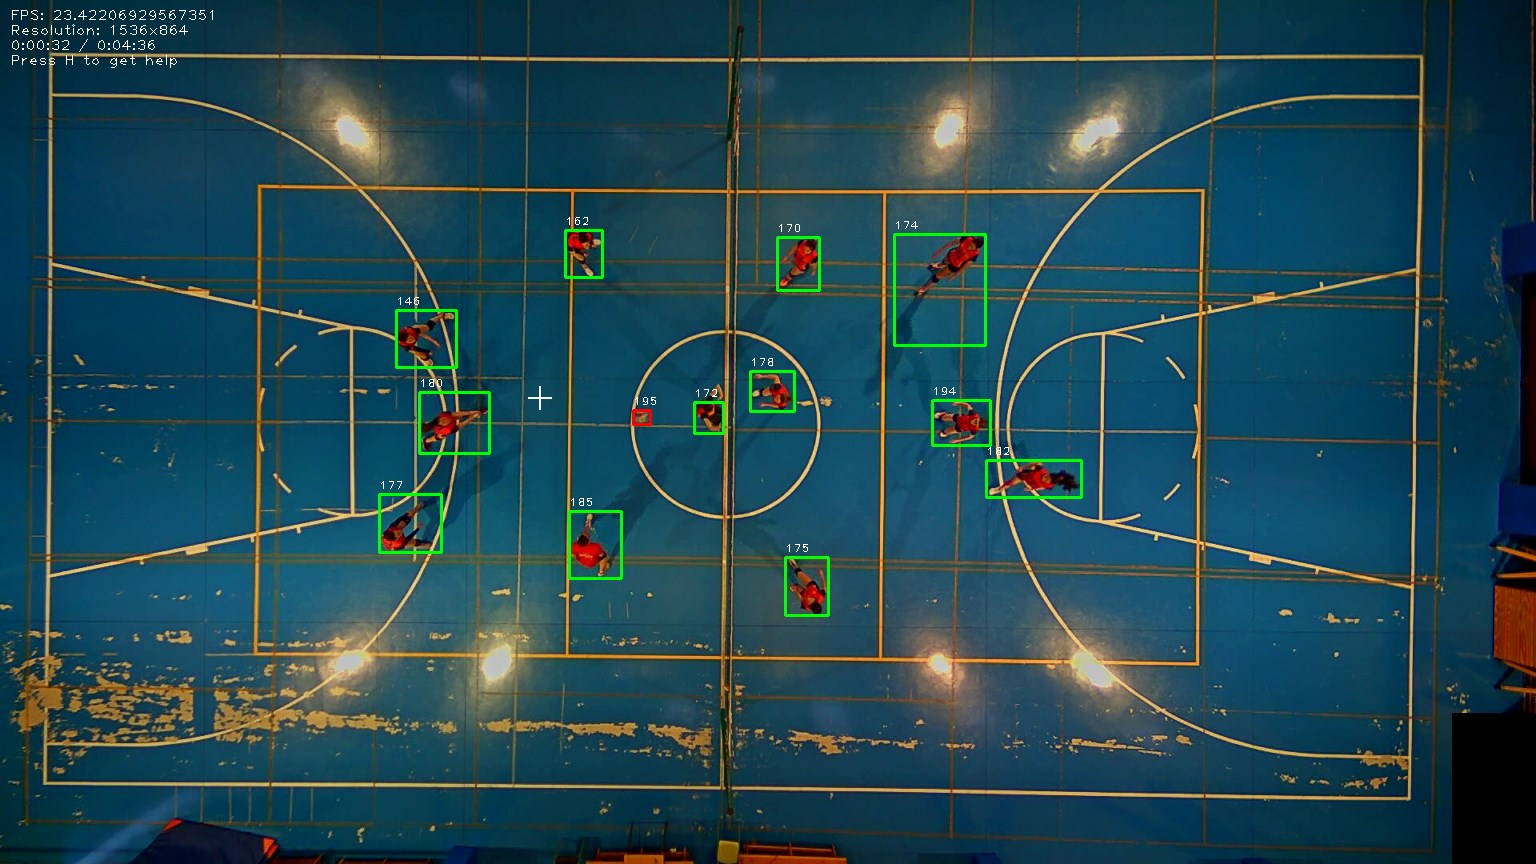
\includegraphics[width=.9\linewidth]{images/MOG}
  \caption { }
  \label{fig:MOG1b}
\end{subfigure}
\caption{Salida del algoritmo MOG (a) Imagen binarizada del algoritmo (b) Imagen del vídeo tras aplicar la máscara }
\label{fig:MOG}
\end{figure}

El funcionamiento de MOG en un frame puede verse en la figura \ref{fig:MOG}, como puede verse, el algoritmo detecta los cuerpos con cierto nivel de fidelidad, aunque en algunos momentos puede ser especialmente sensible a una jugadora estática. Por otro lado, la detección de las sombras no es en absoluto perfecta, y no en pocas ocasiones se marcan partes de la sombra como componentes de la imagen. El rendimiento es correcto, no se aprecian ralentizaciones graves.

\subsubsection*{MOG2}
MOG2 es un algoritmo propuesto en los trabajos \cite{art:Zivkovic1} y \cite{art:Zivkovic2} de Z. Zivkovic.

\subsubsection*{GMG}
GMG surge en un trabajo de Godbehere \textit{et al.} \cite{art:Godbehere}. En este trabajo aclaran los autores que se inspiraron en los algoritmos ya existentes en OpenCV. El método tiene una peculiaridad respecto al resto, y es que requiere de un número $T$ de frames determinado para inicializar el modelo de fondo. Esta inicialización puede ser interesante en caso de contar con vídeos en los que se vea el fondo al principio sin ningún tipo de oclusión, en nuestro caso, que se vea el campo sin ningún jugador. Desgraciadamente, esto no siempre es posible, por lo que la efectividad inicial puede verse limitada debido a esta condición.

Durante la inicialización, se guarda un histograma $\hat{H}_{ij}(k)$ en espacio RGB por cada pixel previamente cuantizado. Los primeros $T$ frames del vídeo se utilizan, como datos de entrenamiento para estimar la función de probabilidad de cada pixel, es decir, el modelo de fondo. El proceso de inicialización comienza en cada frame generando un vector $f_{ij}(k) = L(\hat{I}_{ij}(k)) \in \mathcal{F}$ mediante una función $L$ a partir de la entrada. Una vez generados todos los vectores, se calcula el histograma $\hat{H}_{ij}(T) = \frac{1}{F_{tot}}\Sigma_{x = 1}^T f_{ij}(x)$. $F_{tot}$ es el número total de distintos factores observados, que siempre debe ser menor o igual que $F_{max}$, una constante del sistema. En caso de que sea mayor, se eliminan las observaciones más antiguas hasta que se cumpla que $F_{tot} \leq F_{max}$.

A partir de aquí se utiliza inferencia bayesiana para calcular la probabilidad de que un píxel dado sea fondo a partir del factor observado. Sea $p(F|f)$ la probabilidad de que un pixel con factor $f_{ij}(k)$ sea parte del primer plano y $p(B|f)$ la probabilidad de que este mismo pixel sea fondo:
\[
    p(B|f) = \frac{p(f|B)p(B)}{p(f|B)p(B)+p(f|F)p(F)}
\]

Siendo $p(f|B) = f_{ij}(k)^T\hat{H}_{ij}(k)$, $p(f|F) = 1 - p(f|B)$, $p(F)$ es un parámetro constante que afecta a la sensibilidad del algoritmo y $p(B) = 1 - p(F)$. Una vez calculado $p(B|f)$ para cada pixel, obtenemos una imagen $P(k)$ a la que se le aplican una serie de transformaciones morfológicas de manera que se eliminen las posibles pequeñas formas anómalas que puedan detectarse y las componentes de la imagen aparezcan conectadas. Por último se aplica un umbral a la imagen para generar a partir de ella una imagen en binario que servirá como máscara y será la salida del sustractor.

Por último se debe actualizar el histograma que se usa como modelo de fondo de manera que se adapte a posibles cambios en la escena. Si un pixel esta marcado como frente de la escena, el histograma para él no se actualiza. Si no, si el factor $f_{ij}(k)$ tiene peso 0 en el histograma y se ha excedido la constante $F_max$, se debe eliminar algún factor del histograma, el de menor peso. A continuación se actualiza el histograma con el nuevo factor a añadir: $H_{ij}(k+1)=(1-\alpha)H_{ij}(k)+\alpha f_{ij}(k)$ siendo $\alpha$ el parámetro de adaptación (\textit{learning rate}) del algoritmo, y cuanto más grande sea, antes se eliminan las observaciones anteriores.

\begin{figure}
\begin{subfigure}{.5\textwidth}
  \centering
  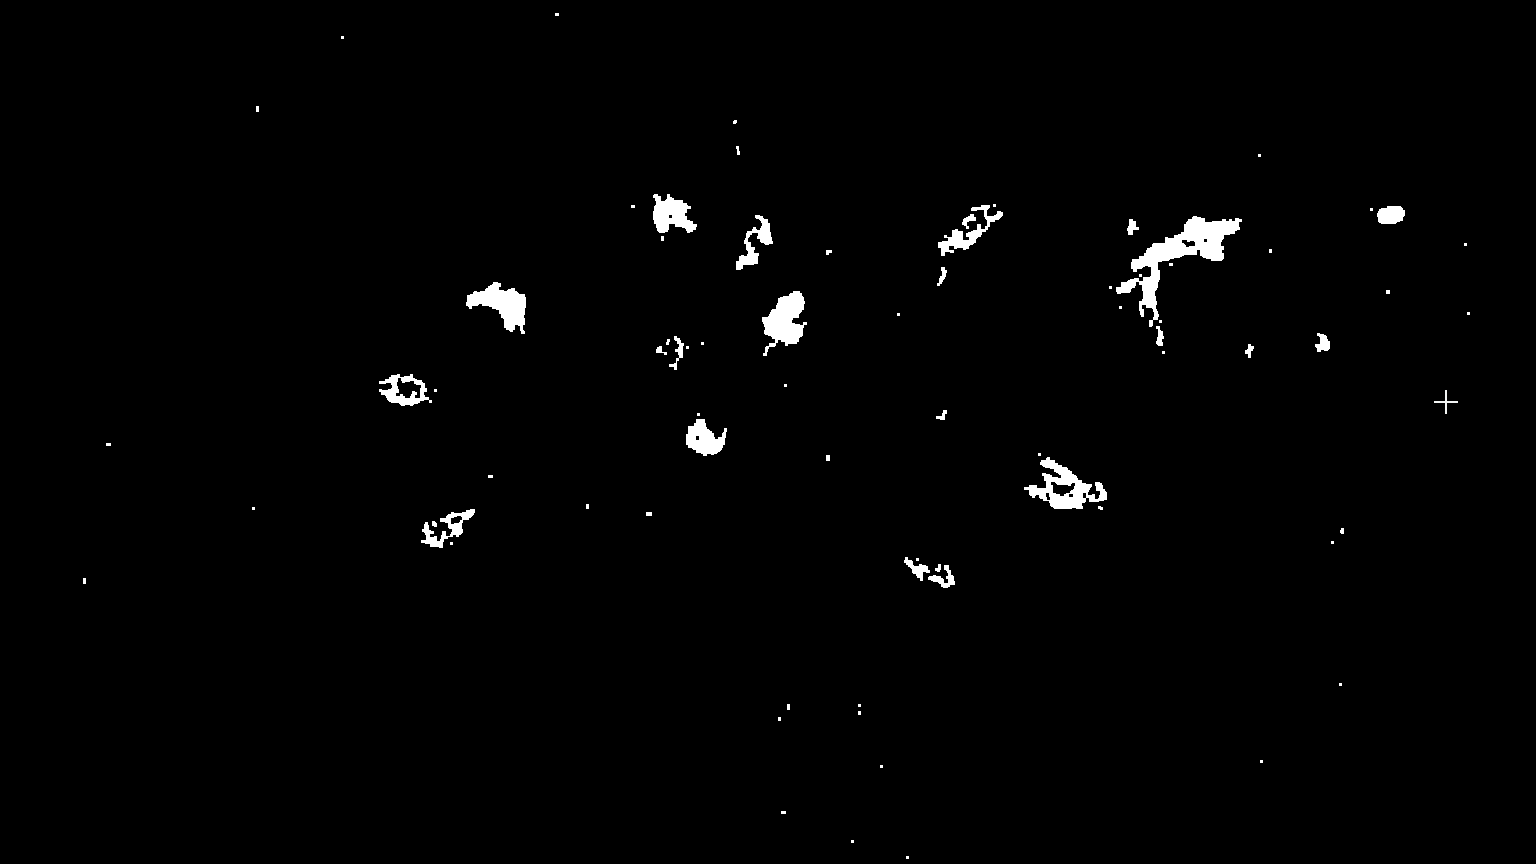
\includegraphics[width=.9\linewidth]{images/GMGsub}
  \caption { }
  \label{fig:GMG1a}
\end{subfigure}%
\begin{subfigure}{.5\textwidth}
  \centering
  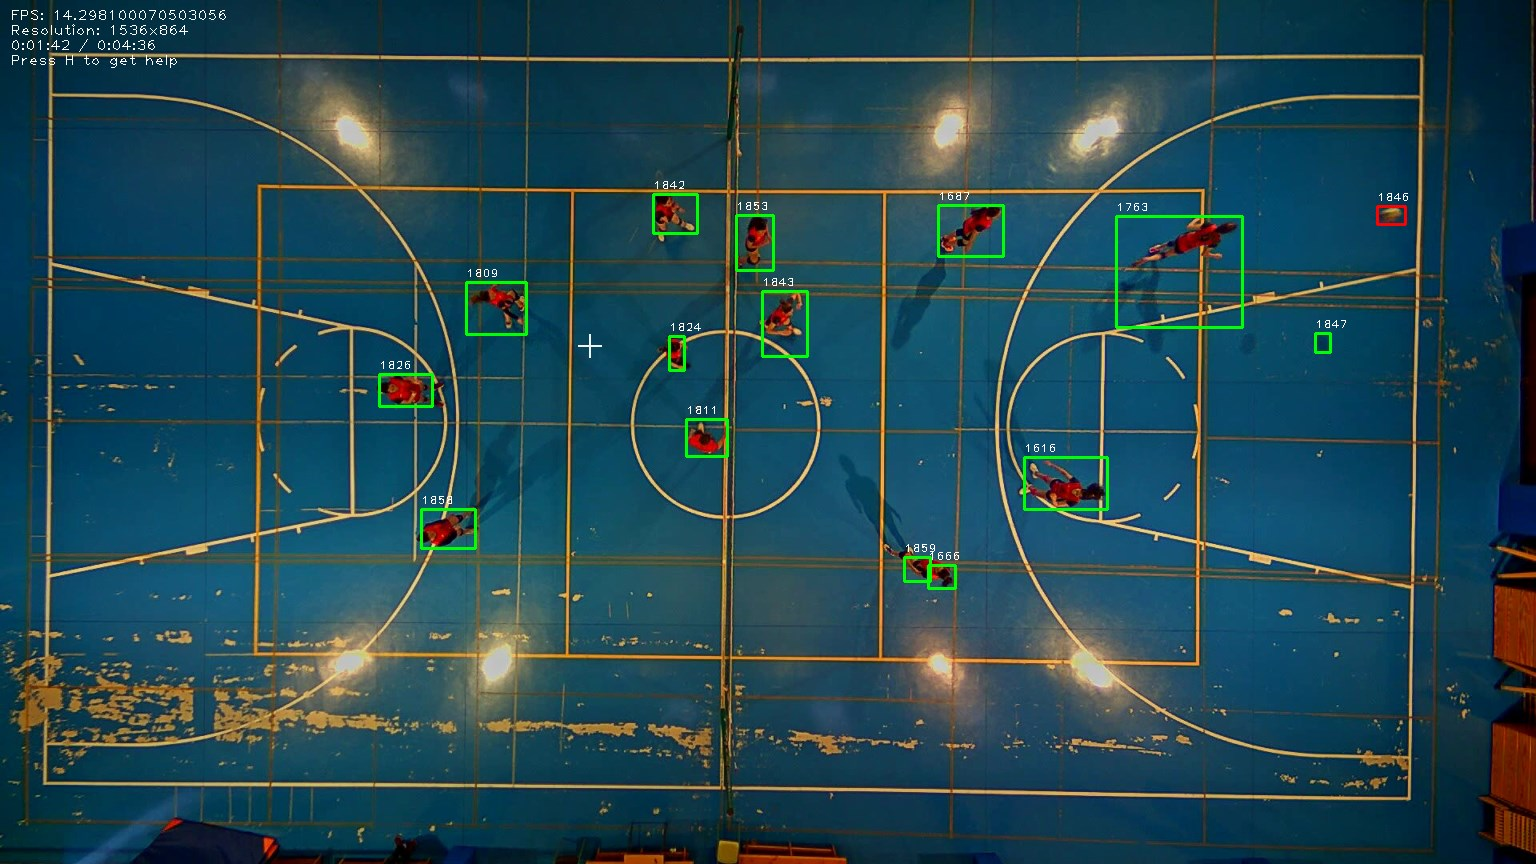
\includegraphics[width=.9\linewidth]{images/GMG}
  \caption { }
  \label{fig:GMG1b}
\end{subfigure}
\caption{Salida del algoritmo GMG (a) Imagen binarizada del algoritmo (b) Imagen del vídeo tras aplicar la máscara }
\label{fig:GMG}
\end{figure}

En cuanto al desempeño del algoritmo, en la figura \ref{fig:GMG} podemos ver que es extremadamente sensible al ruido de la cámara, cosa que hace que la detección de objetos no sea estable. Esta inestabilidad hace que constantemente se pierdan de un frame a otro algunos de los contornos, y haya que asignarles etiquetas nuevas, lo que explica que en la imagen haya etiquetas tan altas. Se aprecian algunos fallos en la detección de sombras, por ejemplo los de la jugadora más arriba a la derecha y el balón en la imagen. 

El rendimiento no es especialmente bueno, y se puede apreciar que cuando el ruido de imagen es muy grande y se detectan muchos contornos falsos, el funcionamiento es extremadamente lento. Además, durante los frames de inicialización, también se notan algunos bajones de FPS. Con todo, estos problemas no son especialmente serios y un reescalado de la imagen bastaría para paliarlos.


\subsubsection*{CNT}
Este método fue desarrollado como open source en \cite{git:CNT}. El algoritmo fue planteado por el desarrollador para que fuera eficiente en máquinas de bajo rendimiento, como raspberryPi. Se basa en ``contar'' (que es de donde viene su nombre) cuántos frames se mantiene estable un pixel, y a mayor estabilidad, mayor probabilidad de que este sea fondo. Para que el algoritmo se comporte bien ante un objeto que desaparece de escena, existe un parámetro para darle un máximo crédito a los pixels demasiado estables, de manera que a partir de cierto número de frames, no incrementando más la estabilidad de dicho pixel.

En mi caso, usando este método, la reproducción del vídeo llega sobradamente a los 30 fps, con lo que puede ser útil si existe la necesidad de que la aplicación funcione en tiempo real. Por otro lado, CNT no detecta sombras muy bien, por lo que en caso de que exista el requisito de detectarlas, puede no ser efectivo. También tiene problemas a la hora de distinguir el balón de una jugadora cualquiera, dado que no detecta las formas del todo bien, y la pelota no pasa el test de circularidad.

\subsubsection*{GSOC}
GSOC fue implementado durante un \textit{Google Summer of Code}, no procede de ningún artículo, sino que parte de un algoritmo existente (LSBP). El funcionamiento de este algoritmo no tiene documentación más allá de aclarar que se basa en ¿¿saliencia de vídeo??

En general, el algoritmo funciona de manera bastante robusta en lo que respecta a detectar formas en la escena, e incluso es capaz de detectar sin grandes problemas las sombras. Sin embargo, no logra detectar el balón de manera consistente, por lo que sería necesario usar algún tipo de algoritmo de tracking en conjunción a este.

Por otro lado, a pesar de su robustez, el algoritmo es el más lento de los que se han probado, lo que lo hace bastante desaconsejable para aplicaciones en tiempo real.

\subsubsection*{KNN}
\cite{art:Zivkovic2}

\subsection{Seguimiento}

\subsection{Interfaz gráfica}


